\section{Sterowanie jednostkami w grze Mount\&Blade (Zofia Sosińska)}\label{chap:mb}

Mount\&Blade jest to gra komputerowa z gatunku cRPG (komputerowa gra fabularna, ang. computer role-playing game) z elementami strategicznymi, stworzona przez turecką firmę TaleWorlds Entertainment i wydana przez Paradox Interactive. W otwartym świecie fikcyjnej krainy Calradia, stylizowanej na czasy średniowieczne, gracz ma pełną dowolność stylu rozgrywki. W jego mocy jest zarówno zbieranie armii i dążenie do zostania królem, jak i zostanie wasalem jednego z władców. Za pomocą dialogów i walk z postaciami gracz buduje unikatową historię.
Jedną z wartych uwagi mechanik, zaimplementowaną w grze Mount\&Blade, jest sterowanie jednostkami służącymi granemu charakterowi. Gracz bezpośrednio kieruje jedynie główną postacią. Podczas walki reszcie może wydawać rozkazy. Poprzez cyfry 0-4 wybiera grupę, do której się odnosi np. łuczników. Następnie przez klawisze F1-F11 wydaje konkretny rozkaz np. odwrót. Sztuczna inteligencja postaci zajmuje się już samym wykonaniem czynności. Gracz nie martwi się, czy jednostki znajdą optymalną drogę, będą celować w przeciwników, czy z nimi walczyć.


\begin{figure}[h!tbp]
    \centering
    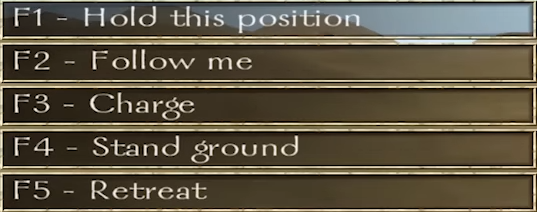
\includegraphics[width=0.9\textwidth]{images/ui/commandsMountBla.png}
    \caption{Wykaz dostępnych rozkazów z gry Mount\&Blade.}\label{fig:MountnBlade}
    \label{fig:mnb}
\end{figure}
